\documentclass{article}

\usepackage{tikz}
\usepackage[inner=0.5cm,outer=0.5cm]{geometry}

\begin{document}

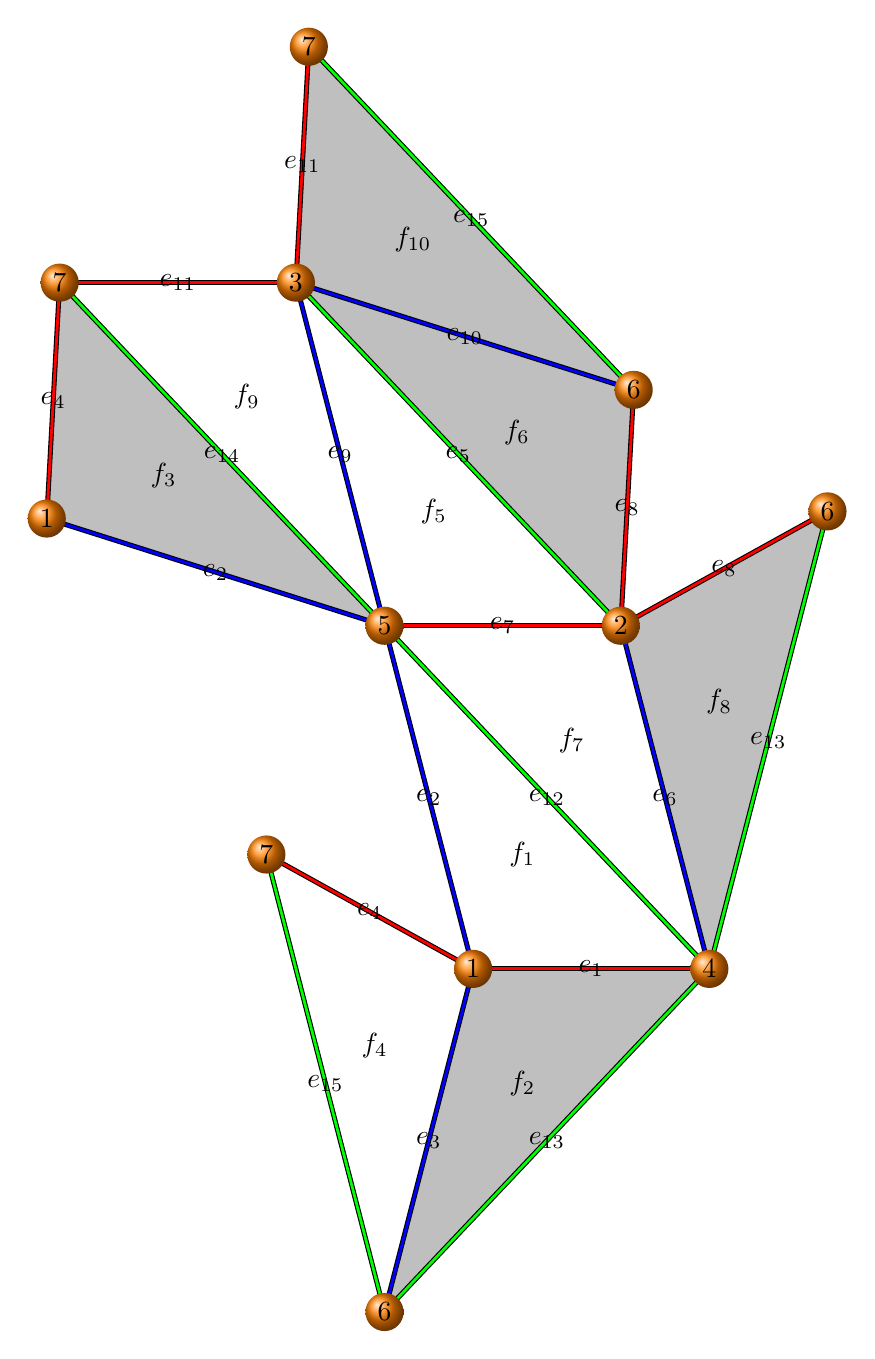
\begin{tikzpicture}[scale=3/2]
\coordinate (V1_1) at (0, 0);
\coordinate (V1_2) at (-3.609375, 3.812467981422927);
\coordinate (V2_1) at (1.25, 2.904737509655563);
\coordinate (V3_1) at (-1.5, 5.809475019311126);
\coordinate (V4_1) at (2, 0);
\coordinate (V5_1) at (-0.75, 2.904737509655563);
\coordinate (V6_1) at (-0.75, -2.904737509655563);
\coordinate (V6_2) at (3, 3.872983346207417);
\coordinate (V6_3) at (1.359375, 4.901744547543762);
\coordinate (V7_1) at (-1.75, 0.9682458365518545);
\coordinate (V7_2) at (-1.390625, 7.806482057199325);
\coordinate (V7_3) at (-3.5, 5.809475019311126);


\fill[white] (V1_1) -- (V4_1) -- (V5_1) -- cycle;
\node (F1) at (0.4166666666666666, 0.9682458365518543) {$f_{1}$};
\fill[lightgray] (V1_1) -- (V4_1) -- (V6_1) -- cycle;
\node (F2) at (0.4166666666666666, -0.9682458365518541) {$f_{2}$};
\fill[lightgray] (V1_2) -- (V5_1) -- (V7_3) -- cycle;
\node (F3) at (-2.619791666666667, 4.175560170129872) {$f_{3}$};
\fill[white] (V1_1) -- (V6_1) -- (V7_1) -- cycle;
\node (F4) at (-0.8333333333333333, -0.6454972243679027) {$f_{4}$};
\fill[white] (V2_1) -- (V3_1) -- (V5_1) -- cycle;
\node (F5) at (-0.3333333333333333, 3.872983346207417) {$f_{5}$};
\fill[lightgray] (V2_1) -- (V3_1) -- (V6_3) -- cycle;
\node (F6) at (0.3697916666666666, 4.538652358836817) {$f_{6}$};
\fill[white] (V2_1) -- (V4_1) -- (V5_1) -- cycle;
\node (F7) at (0.8333333333333333, 1.936491673103709) {$f_{7}$};
\fill[lightgray] (V2_1) -- (V4_1) -- (V6_2) -- cycle;
\node (F8) at (2.083333333333333, 2.25924028528766) {$f_{8}$};
\fill[white] (V3_1) -- (V5_1) -- (V7_3) -- cycle;
\node (F9) at (-1.916666666666667, 4.841229182759271) {$f_{9}$};
\fill[lightgray] (V3_1) -- (V6_3) -- (V7_2) -- cycle;
\node (F10) at (-0.5104166666666665, 6.17256720801807) {$f_{10}$};


\tikzset{EdgeStyle/.style = {thin, double distance=1pt} }

\draw[ EdgeStyle, double=red] (V4_1) -- node { $e_{1}$ } (V1_1);
\draw[ EdgeStyle, double=blue] (V1_1) -- node { $e_{2}$ } (V5_1);
\draw[ EdgeStyle, double=blue] (V5_1) -- node { $e_{2}$ } (V1_2);
\draw[ EdgeStyle, double=blue] (V6_1) -- node { $e_{3}$ } (V1_1);
\draw[ EdgeStyle, double=red] (V7_1) -- node { $e_{4}$ } (V1_1);
\draw[ EdgeStyle, double=red] (V1_2) -- node { $e_{4}$ } (V7_3);
\draw[ EdgeStyle, double=green] (V3_1) -- node { $e_{5}$ } (V2_1);
\draw[ EdgeStyle, double=blue] (V2_1) -- node { $e_{6}$ } (V4_1);
\draw[ EdgeStyle, double=red] (V5_1) -- node { $e_{7}$ } (V2_1);
\draw[ EdgeStyle, double=red] (V2_1) -- node { $e_{8}$ } (V6_2);
\draw[ EdgeStyle, double=red] (V6_3) -- node { $e_{8}$ } (V2_1);
\draw[ EdgeStyle, double=blue] (V5_1) -- node { $e_{9}$ } (V3_1);
\draw[ EdgeStyle, double=blue] (V3_1) -- node { $e_{10}$ } (V6_3);
\draw[ EdgeStyle, double=red] (V3_1) -- node { $e_{11}$ } (V7_2);
\draw[ EdgeStyle, double=red] (V7_3) -- node { $e_{11}$ } (V3_1);
\draw[ EdgeStyle, double=green] (V5_1) -- node { $e_{12}$ } (V4_1);
\draw[ EdgeStyle, double=green] (V4_1) -- node { $e_{13}$ } (V6_1);
\draw[ EdgeStyle, double=green] (V6_2) -- node { $e_{13}$ } (V4_1);
\draw[ EdgeStyle, double=green] (V5_1) -- node { $e_{14}$ } (V7_3);
\draw[ EdgeStyle, double=green] (V6_1) -- node { $e_{15}$ } (V7_1);
\draw[ EdgeStyle, double=green] (V7_2) -- node { $e_{15}$ } (V6_3);



\tikzset{VertexStyle/.style = {
 shape = circle,
 ball color = orange,
 text = black,
 inner sep = 2pt,
 outer sep = 0pt,
 minimum size = 10pt} }

\node[VertexStyle] at (V1_1) {1};
\node[VertexStyle] at (V1_2) {1};
\node[VertexStyle] at (V2_1) {2};
\node[VertexStyle] at (V3_1) {3};
\node[VertexStyle] at (V4_1) {4};
\node[VertexStyle] at (V5_1) {5};
\node[VertexStyle] at (V6_1) {6};
\node[VertexStyle] at (V6_2) {6};
\node[VertexStyle] at (V6_3) {6};
\node[VertexStyle] at (V7_1) {7};
\node[VertexStyle] at (V7_2) {7};
\node[VertexStyle] at (V7_3) {7};

\end{tikzpicture}

\end{document} 
